\documentclass[conference]{IEEEtran}
\usepackage{graphicx}
\usepackage{booktabs}
\usepackage{amsmath,amssymb}
\usepackage{cite}
\usepackage{url}
\usepackage{xcolor}
\newcommand{\NumDays}{183}
\newcommand{\NumMinutes}{263{,}518}
\newcommand{\NumUsable}{158{,}191}
\newcommand{\NumSepMin}{31{,}739}
\newcommand{\NumFlaresAll}{1598}
\newcommand{\NumFlaresC}{1131}
\newcommand{\NumFlaresM}{446}
\newcommand{\NumFlaresX}{21}
\newcommand{\NeuMedian}{0.41}
\newcommand{\NeuN}{372}
\newcommand{\NeuPos}{95}
\newcommand{\FullTSSFifteen}{0.11}
\newcommand{\FullFARFifteen}{0.87}
\newcommand{\FullPODFifteen}{0.42}
\newcommand{\HistTSSFifteen}{0.08}
\newcommand{\FullTSSThirty}{0.08}
\newcommand{\FullFARThirty}{0.76}
\newcommand{\FullPODThirty}{0.38}
\newcommand{\HistTSSThirty}{0.07}
\newcommand{\FullTSSSixty}{0.08}
\newcommand{\FullFARSixty}{0.60}
\newcommand{\FullPODSixty}{0.39}
\newcommand{\HistTSSSixty}{0.08}
\newcommand{\FullTSSMThirty}{0.28}
\newcommand{\FullFARMThirty}{0.90}
\newcommand{\FullPODMThirty}{0.63}
\newcommand{\HistTSSMThirty}{0.18}
\newcommand{\FullTSSMSixty}{0.23}
\newcommand{\FullFARMSixty}{0.84}
\newcommand{\FullPODMSixty}{0.62}
\newcommand{\HistTSSMSixty}{0.22}
\newcommand{\PosYfifteen}{16{,}093}
\newcommand{\PosYthirty}{30{,}641}
\newcommand{\PosYsixty}{55{,}304}
\newcommand{\PosMthirty}{9{,}174}
\newcommand{\PosMsixty}{17{,}297}
\newcommand{\MedFoldSD}{0.06}
\newcommand{\SigAll}{105}
\newcommand{\SigTotal}{51}
\newcommand{\SigSXR}{11}
\newcommand{\SigHXR}{1}
\newcommand{\SigEUV}{7}
\newcommand{\SigSXRHXR}{8}
\newcommand{\SigPerSubset}{15}
\newcommand{\ShapLoSXR}{0.005}
\newcommand{\ShapHiSXR}{0.068}
\newcommand{\ShapLoHXR}{-0.012}
\newcommand{\ShapHiHXR}{0.007}
\newcommand{\ShapLoEUV}{-0.015}
\newcommand{\ShapHiEUV}{0.018}
\newcommand{\HistLoC}{0.05}
\newcommand{\HistHiC}{0.06}
\newcommand{\HistM}{0.17}
\newcommand{\RangeLoC}{0.05}
\newcommand{\RangeHiC}{0.10}
\newcommand{\RangeLoM}{0.15}
\newcommand{\RangeHiM}{0.25}
\newcommand{\LevelMThirty}{0.27}
\newcommand{\LevelMSixty}{0.28}
\newcommand{\FARlo}{0.60}
\newcommand{\FARhi}{0.90}
\newcommand{\NumFlaresEvalC}{1085}
\newcommand{\NumFlaresEvalM}{319}
\newcommand{\PairNC}{16}
\newcommand{\PairMedC}{-1.0}
\newcommand{\PairEarlyC}{56}
\newcommand{\PairSameC}{12}
\newcommand{\PairLateC}{31}
\newcommand{\PairNMX}{146}
\newcommand{\PairMedMX}{-1.0}
\newcommand{\PairEarlyMX}{55}
\newcommand{\PairSameMX}{25}
\newcommand{\PairLateMX}{21}
\newcommand{\SepMeanAbs}{0.015}
\newcommand{\SepMaxAbs}{0.040}
\newcommand{\SepShapLoSXR}{0.003}
\newcommand{\SepShapHiSXR}{0.082}
\newcommand{\SepShapLoHXR}{-0.006}
\newcommand{\SepShapHiHXR}{0.003}
\newcommand{\SepShapLoEUV}{-0.005}
\newcommand{\SepShapHiEUV}{0.017}
\newcommand{\FwdDiffMean}{0.02}
\newcommand{\FwdShareLower}{78}
\newcommand{\MagGainLoo}{-0.006}
\newcommand{\MagGainFwd}{-0.004}
\newcommand{\LevelLoo}{0.14}
\newcommand{\LevelFwd}{0.11}
\newcommand{\HistLooBlocks}{0.15}
\newcommand{\HistFwd}{0.13}
\newcommand{\FwdGainSXR}{0.046}
\newcommand{\FwdGainHXR}{0.001}
\newcommand{\FwdGainEUV}{0.004}
\newcommand{\FwdGainSXRHXR}{0.052}
\newcommand{\FwdGainSXREUV}{0.036}
\newcommand{\FwdGainHXREUV}{-0.001}
\newcommand{\FwdGainSXRHXREUV}{0.039}
\newcommand{\PairGainSXR}{0.044}
\newcommand{\PairGainHXR}{0.003}
\newcommand{\PairGainEUV}{0.012}
\newcommand{\PairGainSXRHXR}{0.041}
\newcommand{\PairGainSXREUV}{0.047}
\newcommand{\PairGainHXREUV}{0.013}
\newcommand{\PairGainSXRHXREUV}{0.043}
\newcommand{\PairGainHISTONLY}{0.008}
\newcommand{\PairSigTotal}{40}
\newcommand{\PairSigAll}{105}
\newcommand{\FwdSigTotal}{5}
\newcommand{\FwdSigAll}{70}
\newcommand{\CausalRowsMin}{160{,}559}
\newcommand{\CausalFeatures}{92}
\newcommand{\CausalCuts}{3}
\newcommand{\CausalMaxDiff}{0}
\newcommand{\EpDayFullLo}{11}
\newcommand{\EpDayFullHi}{18}
\newcommand{\EpPrecFullLo}{32}
\newcommand{\EpPrecFullHi}{61}
\newcommand{\EpDayHistLo}{6}
\newcommand{\EpDayHistHi}{8}
\newcommand{\EpPrecHistLo}{69}
\newcommand{\EpPrecHistHi}{78}
\newcommand{\DutyLo}{31}
\newcommand{\DutyHi}{47}
\newcommand{\FwdTSSCLo}{-0.02}
\newcommand{\FwdTSSCHi}{0.13}
\newcommand{\FwdTSSMLo}{0.18}
\newcommand{\FwdTSSMHi}{0.30}
\newcommand{\FwdShapLoSXR}{-0.013}
\newcommand{\FwdShapHiSXR}{0.068}
\newcommand{\FwdShapLoHXR}{-0.005}
\newcommand{\FwdShapHiHXR}{0.008}
\newcommand{\FwdShapLoEUV}{-0.024}
\newcommand{\FwdShapHiEUV}{0.011}

\makeatletter
\newcommand{\absval}[1]{\expandafter\@gobble#1}
\makeatother
\graphicspath{{figs/}}

\begin{document}

\title{Quantifying the Predictive Contribution of Hard X-ray, Soft X-ray, and EUV Observations for Early Solar Flare Forecasting: Evidence from Aditya-L1}

\author{\IEEEauthorblockN{Ashritha Abbabathula}
\IEEEauthorblockA{Vellore Institute of Technology, Chennai, India}}

\maketitle

\begin{abstract}
A few minutes of warning before a solar flare can help operators of HF radio links, satellite navigation and spacecraft. What is less clear is how much each part of the flare spectrum helps with that warning. We put together Aditya-L1 SoLEXS soft X-ray (SXR) and HEL1OS hard X-ray (HXR) light curves, GOES extreme-ultraviolet (EUV) irradiances, SDO/HMI magnetic-field summaries and NOAA flare labels for \NumDays\ days (1~July to 31~December 2024, \NumFlaresAll\ flares of class C or above), and we ask two separate questions. The first is forecasting: beyond recent flare history and the magnetic state of the Sun, how much does each band add when predicting a flare 15 to 60 minutes ahead? The second is nowcasting: how soon does each band show a flare that is already happening? We test three model families, every band combination and two time-series validation designs, and split the credit between bands with exact Shapley values. The skill we find is small. The True Skill Statistic (TSS) is \RangeLoC--\RangeHiC\ for C-class-and-above targets and \RangeLoM--\RangeHiM\ for M-class-and-above targets. Testing forward in time lowers it by \FwdDiffMean\ on average compared with leave-one-block-out (the drop was larger in a two-month pilot). Magnetic summaries add nothing we can detect. SXR is the only band that helps consistently, mostly for M+ targets (Shapley value around 0.05--0.07 TSS), but a single SoLEXS-level feature does just as well, so most of this is persistence. HXR, even with sub-minute features, and EUV give no steady gain. At the TSS-optimal threshold an alert is active \DutyLo--\DutyHi\% of the time. The nowcasting result is the clearer one: in \NeuPos\% of \NeuN\ M/X flares HEL1OS follows the SXR derivative (median rank correlation \NeuMedian, the Neupert effect), and when both instruments detect a flare, HEL1OS registers it a median of \absval{\PairMedMX}~minute before SoLEXS.
\end{abstract}

\begin{IEEEkeywords}
solar flares, Aditya-L1, SoLEXS, HEL1OS, hard X-ray, space-weather forecasting, Neupert effect, Shapley values
\end{IEEEkeywords}

\section{Introduction}
Within minutes, a solar flare can release a huge amount of magnetic energy in the corona and disturb HF communication, satellite navigation and spacecraft. Routine monitoring relies on the GOES soft X-ray flux, which is also what defines the flare classes C, M and X. A flare, though, shines across the whole spectrum, and each band reflects different physics. Hard X-rays (HXR) come from non-thermal electrons and mark the impulsive release of energy. Soft X-rays (SXR) follow the heated plasma. Extreme-ultraviolet (EUV) lines come from the chromosphere and transition region. The Neupert effect ties the first two together: the HXR light curve looks like the time derivative of the SXR one~\cite{neupert1968,dennis1993,veronig2002}.

This leads to a practical question: \emph{if we want a short-notice flare forecast, how much does each band add, alone or combined, beyond what recent flaring and the magnetic state of the Sun already tell us?} The question matters because a band can look useful simply because it tracks ``an active region is flaring a lot'', and flare history gives that for free. Aditya-L1~\cite{tripathi2022} makes a fair comparison possible. It carries SoLEXS (soft X-rays) and HEL1OS (hard X-rays, 8--150~keV)~\cite{nandi2025} and watches the Sun without interruption from the first Sun--Earth Lagrange point.

We treat two tasks separately, since they are easy to mix up. \emph{Forecasting} means predicting the start of a flare that has not happened yet. \emph{Nowcasting} means spotting a flare that is already under way, and asking how early. This paper makes five contributions: (i)~a reproducible one-minute multi-band dataset and a causal feature set for \NumDays\ days of Aditya-L1 data, with an automated test showing that no feature uses future data; (ii)~a controlled comparison of all band combinations over three model families and five targets, against a baseline of flare history and magnetic state, under two validation designs; (iii)~an exact Shapley split of forecast skill by band, with two ways of estimating uncertainty; (iv)~alert-level metrics that show what the forecasts would be like in use; and (v)~an analysis of detection latency by band for nowcasting. We report what we found, and the honest summary is that the forecast gains from the emission bands are small and fragile, while the clearest findings are about nowcasting.

\section{Related Work}
\textbf{Forecasting from magnetic data.} The most skilful flare forecasts mostly rely on photospheric magnetic-field measurements.  Bobra and Couvidat~\cite{bobra2015} classified flaring regions from SDO/HMI vector-field parameters, and Chen \emph{et al.}~\cite{chen2019} used time series of such parameters and magnetogram sequences to study precursors. Comparisons across methods rely on skill scores such as the TSS~\cite{bloomfield2012,barnes2016}.

\textbf{Forecasting from X-ray series.} Landa and Reuveni~\cite{landa2022} trained a one-dimensional convolutional network on GOES X-ray time series to estimate M- and X-class flare probabilities over horizons of 1--96~hours, comparing random and chronological splits. So an X-ray series from one band does carry some forecast information. What that work does not ask is how much \emph{extra} the other bands give on top of such a series, or on top of flare history.

\textbf{Precursors.} Statistical work on precursor flares~\cite{gyenge2016} and on hot soft X-ray onsets before the hard X-ray burst~\cite{hudson2021} shows that weak signals can precede the impulsive phase, and early Aditya-L1 results using SUIT together with SoLEXS and HEL1OS have reported small pre-flare brightenings clustered where major flares later occurred~\cite{isro2026}. Whether these precursors turn into usable forecast skill at the cadences we have here is still an open question.

\textbf{The Neupert effect.} Veronig \emph{et al.}~\cite{veronig2002} found that about half of 1\,114 flares followed the Neupert relation and about a quarter deviated strongly; HEL1OS and SoLEXS now allow the test on a single platform.

\textbf{Gap.} In the sources we looked at (a targeted search, not a full review), we found no study that compares the incremental forecast contribution of SXR, HXR and EUV under one protocol on Aditya-L1 data, with explicit flare-history and magnetic-state baselines and forward-in-time validation. This paper is an exploratory attempt at that comparison, plus a separate nowcasting analysis.

\section{Data}
\begin{table}[t]
\caption{Data used}
\label{tab:data}
\centering\footnotesize
\resizebox{\columnwidth}{!}{\begin{tabular}{lll}
\toprule
Band & Instrument & Product used \\
\midrule
SXR & Aditya-L1 SoLEXS (SDD2) & Level-1 light curve, 1 s $\rightarrow$ 1 min \\
HXR & Aditya-L1 HEL1OS CZT1+2 & 20--40, 40--60, 60--150 keV, $\approx$8 s readout $\rightarrow$ 1 min \\
EUV & GOES-16 EUVS & 25.6, 28.4, 30.4 nm lines, 1 min \\
Labels & GOES-16 XRS & NOAA flare summary (C, M, X) \\
\bottomrule
\end{tabular}
}
\end{table}

\textbf{SXR.} SoLEXS Level-1 light curves (detector SDD2) at 1~s cadence, averaged to one minute when at least 30 valid seconds are present; otherwise the minute is missing. \textbf{HXR.} HEL1OS Level-1 light curves from the two CZT detectors, summed over detectors in three bands, 20--40, 40--60 and 60--150~keV (the last is the sum of the 60--80 and 80--150~keV bands). The files are time-stamped at 1~s, but inspection shows that a reading arrives only about every 8~s (83\% of samples are zero, and the values equal their squared errors, i.e.\ they are raw counts); the one-minute means (counts per second) are unaffected, and all sub-minute features use 8~s blocks. Where several processing versions exist, the newest is used. \textbf{EUV.} GOES-16 EUVS irradiances at 25.6, 28.4 and 30.4~nm at one-minute cadence, with quality flags applied. \textbf{Magnetic state.} SDO/HMI SHARP parameters~\cite{scherrer2012,bobra2014} from the JSOC keyword service at 12-minute cadence, reduced to full-disk summaries (sums of unsigned flux, current helicity and free-energy proxy, the largest R-value, number of regions) over good-quality regions within $60^{\circ}$ of the central meridian; a value is used only 12 minutes after its observation and carried forward for at most an hour. \textbf{Labels.} Flare start, peak, end and class come from the NOAA GOES-16 XRS flare summary. All series are floored to UTC minutes and aligned on a common one-minute grid; no gap is interpolated. Because labels derive from GOES XRS and the SXR features from SoLEXS, the two are independent instruments observing the same emission.

The window is 1~July to 31~December 2024 (\NumDays\ days) with \NumFlaresAll\ flares of class C or above (\NumFlaresC\ C, \NumFlaresM\ M, \NumFlaresX\ X). Observation gaps, minutes inside an ongoing flare, and periods of solar-energetic-particle (SEP) contamination leave \NumUsable\ usable one-minute samples. The HEL1OS SEP catalogue~\cite{sepcat} lists seven contamination periods in the window (\NumSepMin\ minutes); it describes them as a diagnostic flag, so we exclude them in the main analysis and test the effect of including them (Section~\ref{sec:robust}).

\section{Methods}
\subsection{Features and causality}
Features at minute $t$ use only samples at or before $t$: all rolling windows are right-aligned and all differences look backwards. A feature is missing if any input in its window is missing, and rows with any missing feature are dropped. For each channel we compute the log level (for HXR, the excess over a three-hour running median), changes over the previous 5, 15 and 30 minutes, a curvature term, rolling standard deviations over 15 and 60 minutes, and the distance below the 60-minute running maximum. The HXR block adds the 60--150/20--40~keV hardness and sub-minute features from the 8~s blocks (peak block rate relative to the minute mean, within-minute variability, and a count of blocks above a Poisson threshold, with 15-minute totals). A \emph{Neupert} block, included only when both SXR and HXR are present, encodes the relation between the standardised HXR excess and the fractional SXR derivative. A \emph{flare-history} block (C+ flares in the previous 6 and 24 hours, hours since the last flare ended, the largest recent peak flux, and recent M+ flares; only flares already ended by $t$) and a \emph{magnetic} block (the full-disk summaries and their 6- and 24-hour changes) are present in \emph{every} band configuration, and together form the baseline against which the bands are measured. A separate ``history only'' model without the magnetic block shows what the magnetic features themselves add.

We verify causality directly. For \CausalCuts\ cut times we deleted all data after the cut, recomputed every feature, and compared with the full computation on all rows up to the cut. Across at least \CausalRowsMin\ rows and all \CausalFeatures\ features the maximum difference was \CausalMaxDiff, so no feature depends on later data.

\subsection{Targets}
The targets are binary: \emph{a new flare of class $\ge$C (or $\ge$M) starts within the next $H$ minutes}, $H\in\{15,30,60\}$ for C+ and $H\in\{30,60\}$ for M+. Minutes inside an ongoing flare are excluded, so the task is to forecast onset. This exclusion uses the flare's end time, which a live system would learn only after detecting the flare, and so gives a small hindsight advantage (Section~\ref{sec:disc}). Positive rates are \PosYfifteen, \PosYthirty\ and \PosYsixty\ minutes for the C+ horizons and \PosMthirty\ and \PosMsixty\ for M+.

\subsection{Validation, models and thresholds}
The usable period is cut into eight contiguous blocks. We use two designs. \emph{Leave-one-block-out (LOO):} each block is the test set once, the following block is the validation set used only to choose the alert threshold (maximising TSS), and all remaining blocks train the model, including later ones. \emph{Forward-in-time:} test block $k$ is predicted by a model trained only on blocks before $k-1$, with block $k-1$ used for the threshold; this covers blocks 3--8. A 60-minute purge gap surrounds the test and validation blocks in both designs, and every fourth training minute is used. Models are elastic-net logistic regression, a random forest (200 trees) and gradient-boosted trees (depth 3, learning rate 0.05, at most 300 rounds with early stopping on the validation block), each with class weights. Standardisation parameters, the penalty strength (by contiguous cross-validation inside the training data) and the threshold are all obtained without the test block. LOO uses all three families; the slower forward design uses logistic regression and boosted trees. Test predictions are pooled across blocks.

\subsection{Metrics}
We report the TSS (probability of detection minus probability of false detection, insensitive to class imbalance). For alerts, minutes above the threshold separated by at most five minutes are merged into \emph{episodes}; an episode is correct if a flare starts after its beginning and within $H$ minutes of its end. We report episodes per day, the share of episodes that are correct (precision), the share of flares preceded by an alert in $[s-H,s)$ for flare start $s$, and the fraction of minutes during which an alert is active. Threshold selection optimises minute-level TSS only.

\subsection{Band attribution}
For each target and model, $v(S)$ is the pooled out-of-sample TSS of the model that uses the baseline (flare history and magnetic state) plus the bands in $S\subseteq\{\mathrm{SXR},\mathrm{HXR},\mathrm{EUV}\}$, and $v(\emptyset)$ is the baseline model. The exact Shapley value~\cite{shapley1953} $\phi_b=\sum_{S\subseteq B\setminus\{b\}}\frac{|S|!\,(|B|-|S|-1)!}{|B|!}\,[v(S\cup\{b\})-v(S)]$ is the band's average marginal contribution, and $\sum_b\phi_b=v(B)-v(\emptyset)$. We use two uncertainty estimates. A block bootstrap (500 resamples of six-hour blocks of the pooled predictions) captures test-set variability but holds the fitted models fixed. A \emph{paired-block} analysis computes, in each test block, the difference in TSS from the baseline model; because each block is a separate refit on a disjoint period, the spread across blocks includes training variability. All comparisons are exploratory and uncorrected for multiplicity. Shapley values are summarised as the mean over model families.

\subsection{Nowcasting detection latency}
For each band we compute a robust $z$-score of the log rate against the median and median absolute deviation of the preceding three hours (lagged five minutes). A flare is \emph{detected} in a band at the first minute within $[$start$-20$~min, peak$]$ with $z>5$ for two consecutive minutes; latency is that time minus the NOAA flare start. Flares inside SEP periods are excluded.

\section{Results}
\subsection{Multi-band behaviour and the Neupert effect}
Fig.~\ref{fig:flare} shows the strongest flare in the window. The HEL1OS burst sits inside the steep rise of the SoLEXS curve and is over before the soft X-ray peak. The EUV lines react more gradually. In the hour before the flare, none of the bands shows an obvious precursor. Across the \NeuN\ M/X flares with complete data, the median per-flare Spearman correlation between HEL1OS 20--40~keV and the SoLEXS derivative during the rise is \NeuMedian, positive in \NeuPos\% of flares (Fig.~\ref{fig:neupert}).

\begin{figure}[t]
\centering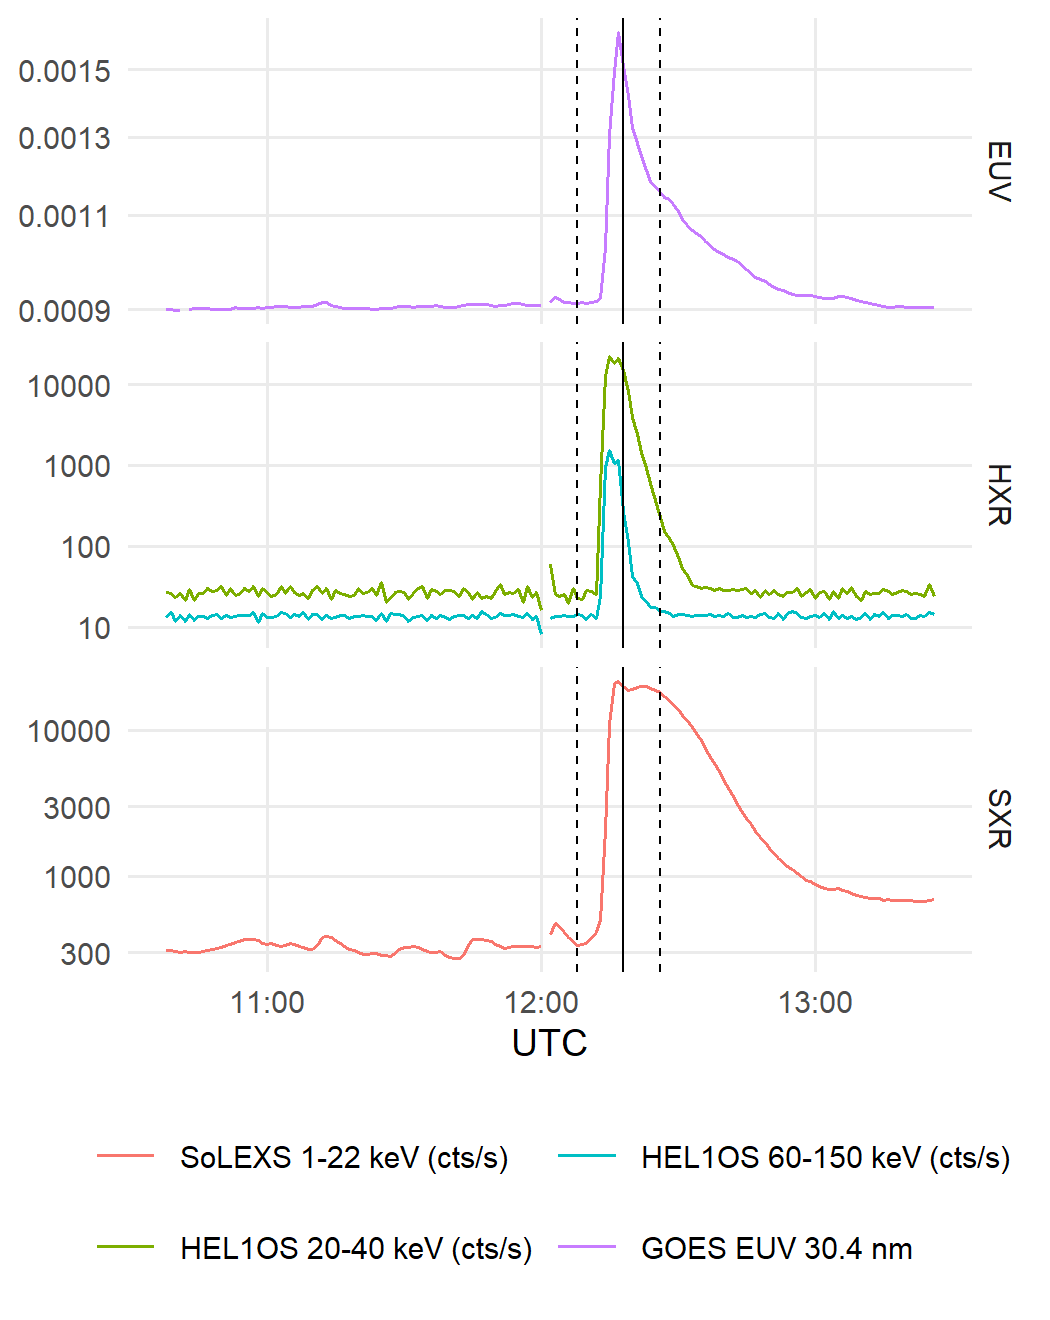
\includegraphics[width=\columnwidth]{fig_example_flare.png}
\caption{Multi-band light curves of the strongest flare in the window. Dashed lines: NOAA start and end; solid: peak.}
\label{fig:flare}
\end{figure}

\begin{figure}[t]
\centering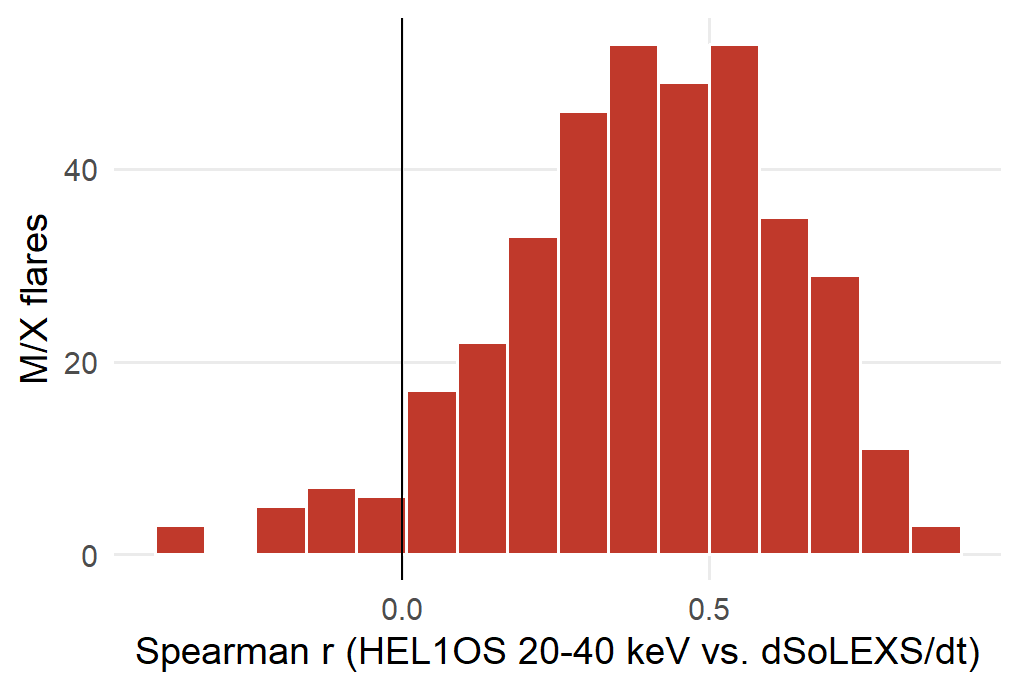
\includegraphics[width=0.92\columnwidth]{fig_neupert.png}
\caption{Per-flare rank correlation between HEL1OS 20--40~keV and dSoLEXS$/dt$ during the rise of M/X flares.}
\label{fig:neupert}
\end{figure}

\subsection{Nowcasting: which band registers a flare first}
Table~\ref{tab:nowcast} and Fig.~\ref{fig:latency} summarise detection. For M/X flares, SoLEXS and HEL1OS 20--40~keV detect similar fractions before the peak, while the 60--150~keV band and the one-minute EUV line rarely exceed the threshold. On the \PairNMX\ M/X flares that both SoLEXS and HEL1OS 20--40~keV detect, HEL1OS detects earlier in \PairEarlyMX\%, in the same minute in \PairSameMX\% and later in \PairLateMX\%, a median difference of \PairMedMX\ minute. Keep in mind that this is a nowcasting result. It only covers flares that are already under way and that both instruments detect, and it is measured against a NOAA start time that itself lags the physical onset. For C-class flares the HXR signal rarely rises above background and SoLEXS is the only band that detects a sizeable fraction.

\begin{table}[t]
\caption{Detection of flares before peak, by band. Latency is relative to the NOAA flare start (positive: after).}
\label{tab:nowcast}
\centering\footnotesize
\begin{tabular}{llrrr}
\toprule
Class & Band & $n$ & Detected & Median [IQR] (min) \\
\midrule
C & SoLEXS & 855 & 29\% & 5.0 [1.0, 7.0] \\
C & HEL1OS 20--40 keV & 855 & 5\% & 4.0 [2.0, 5.0] \\
C & HEL1OS 60--150 keV & 855 & 1\% & 0.0 [-15.5, 4.0] \\
C & GOES EUV 30.4 nm & 844 & 0\% & -- \\
M/X & SoLEXS & 369 & 58\% & 6.0 [3.0, 8.0] \\
M/X & HEL1OS 20--40 keV & 369 & 58\% & 5.0 [3.0, 7.0] \\
M/X & HEL1OS 60--150 keV & 369 & 16\% & 7.0 [3.5, 8.0] \\
M/X & GOES EUV 30.4 nm & 366 & 0\% & 7.0 [7.0, 7.0] \\
\bottomrule
\end{tabular}

\end{table}

\begin{figure}[t]
\centering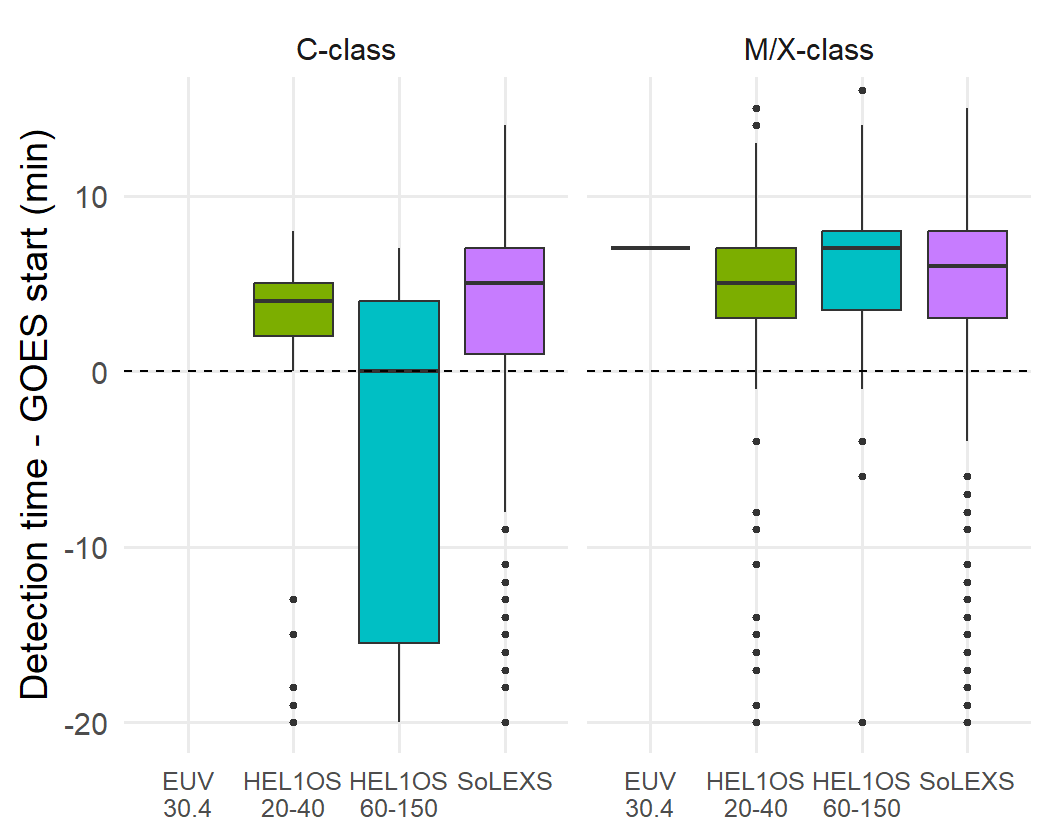
\includegraphics[width=\columnwidth]{fig_nowcast_latency.png}
\caption{Detection time relative to the NOAA flare start, by band and flare class.}
\label{fig:latency}
\end{figure}

\subsection{Forecasting skill under two validation designs}
Table~\ref{tab:skill} gives the pooled TSS under leave-one-block-out and Table~\ref{tab:forward} under forward-in-time evaluation (mean of model families). On the same test blocks the forward design gives lower TSS in \FwdShareLower\% of configurations, by \FwdDiffMean\ on average (the baseline falls from \HistLooBlocks\ to \HistFwd). This gap is much smaller than the 0.11 we saw in a pilot on the last two of these months. So leave-one-block-out is less optimistic when there is more data, though it is still somewhat optimistic. For M+ targets a single SoLEXS-level feature reaches \LevelMThirty\ and \LevelMSixty\ under LOO and 0.29 and 0.28 forward in time, as high as any band combination, whereas it has no skill for C+ targets: for the larger flares, most of the skill is the persistence of the current soft X-ray level. The magnetic features themselves add \MagGainLoo\ (LOO) and \MagGainFwd\ (forward) TSS to flare history, i.e.\ nothing detectable. The fold-to-fold standard deviation of the TSS (median \MedFoldSD) is comparable to many differences between neighbouring rows, so small differences should not be over-read.

\begin{table}[t]
\caption{Pooled TSS, leave-one-block-out (mean of three model families). All rows except the last include flare history; ``History + magnetic'' is the baseline.}
\label{tab:skill}
\centering\footnotesize
\begin{tabular}{lccccc}
\toprule
Features & C+ 15 & C+ 30 & C+ 60 & M+ 30 & M+ 60 \\
\midrule
History + magnetic & 0.06 & 0.05 & 0.05 & 0.16 & 0.18 \\
+SXR & 0.10 & 0.08 & 0.06 & 0.22 & 0.25 \\
+HXR & 0.06 & 0.06 & 0.06 & 0.17 & 0.18 \\
+EUV & 0.10 & 0.09 & 0.07 & 0.19 & 0.16 \\
+SXR+HXR & 0.09 & 0.07 & 0.06 & 0.23 & 0.23 \\
+SXR+EUV & 0.10 & 0.10 & 0.07 & 0.23 & 0.24 \\
+HXR+EUV & 0.08 & 0.07 & 0.07 & 0.18 & 0.15 \\
+SXR+HXR+EUV & 0.09 & 0.08 & 0.08 & 0.23 & 0.22 \\
History only (no magnetic) & 0.05 & 0.05 & 0.05 & 0.17 & 0.17 \\
\midrule
SoLEXS level only & 0.03 & 0.03 & 0.02 & 0.27 & 0.28 \\
\bottomrule
\end{tabular}

\end{table}

\begin{table}[t]
\caption{Pooled TSS, forward-in-time (blocks 3--8; mean of logistic and boosted-tree families).}
\label{tab:forward}
\centering\footnotesize
\begin{tabular}{lccccc}
\toprule
Features & C+ 15 & C+ 30 & C+ 60 & M+ 30 & M+ 60 \\
\midrule
History + magnetic & 0.09 & 0.07 & 0.11 & 0.20 & 0.19 \\
+SXR & 0.13 & 0.08 & 0.08 & 0.28 & 0.26 \\
+HXR & 0.08 & 0.07 & 0.09 & 0.19 & 0.19 \\
+EUV & 0.10 & 0.09 & 0.08 & 0.23 & 0.21 \\
+SXR+HXR & 0.12 & 0.10 & 0.10 & 0.30 & 0.28 \\
+SXR+EUV & 0.11 & 0.09 & 0.06 & 0.29 & 0.26 \\
+HXR+EUV & 0.10 & 0.08 & 0.08 & 0.24 & 0.20 \\
+SXR+HXR+EUV & 0.13 & 0.08 & 0.08 & 0.28 & 0.26 \\
\midrule
History only (no magnetic) & 0.08 & 0.09 & 0.12 & 0.18 & 0.20 \\
SoLEXS level only & 0.01 & -0.02 & -0.01 & 0.29 & 0.28 \\
\bottomrule
\end{tabular}

\end{table}

\subsection{Contribution of each band}
Table~\ref{tab:paired} compares each band subset with the baseline block by block. Under LOO, SXR-containing sets gain about 0.04--0.05 TSS (\PairGainSXR\ for SXR alone) while HXR alone gains \PairGainHXR\ and EUV alone \PairGainEUV, and \PairSigTotal\ of the \PairSigAll\ (target, model, subset) intervals lie above zero, almost all of them for SXR-containing sets. Under forward evaluation the corresponding gains are \FwdGainSXR\ for SXR and \FwdGainSXRHXR\ for SXR+HXR; the full model gains \FwdGainSXRHXREUV, HXR alone \FwdGainHXR\ and EUV alone \FwdGainEUV, and just \FwdSigTotal\ of \FwdSigAll\ intervals exceed zero (with six blocks the power is low). Table~\ref{tab:shapley2} shows the Shapley contributions across targets (ranges \FwdShapLoSXR\ to \FwdShapHiSXR\ for SXR, \FwdShapLoHXR\ to \FwdShapHiHXR\ for HXR and \FwdShapLoEUV\ to \FwdShapHiEUV\ for EUV under forward evaluation). So SXR is the only band that consistently helps beyond flare history and magnetic state; it is largest for M+ targets (Shapley 0.05--0.07 in both designs), but because a one-feature SoLEXS-level model matches it, we read it as persistence rather than as precursor information. HXR and EUV add no consistent contribution in these data, and the forward-in-time intervals are wide (six blocks).

\begin{table}[t]
\caption{Mean TSS gain over the baseline model, averaged over paired test blocks and model families; CI$>0$: number of (target, model) intervals whose 95\% $t$-interval lies above zero.}
\label{tab:paired}
\centering\footnotesize
\begin{tabular}{lcccc}
\toprule
Features & LOO gain & CI$>0$ & Fwd gain & CI$>0$ \\
\midrule
+SXR & 0.044 & 10/15 & 0.046 & 0/10 \\
+HXR & 0.003 &  0/15 & 0.001 & 0/10 \\
+EUV & 0.012 &  3/15 & 0.004 & 0/10 \\
+SXR+HXR & 0.041 &  9/15 & 0.052 & 2/10 \\
+SXR+EUV & 0.047 &  9/15 & 0.036 & 2/10 \\
+HXR+EUV & 0.013 &  1/15 & -0.001 & 0/10 \\
+SXR+HXR+EUV & 0.043 &  8/15 & 0.039 & 1/10 \\
\bottomrule
\end{tabular}

\end{table}

\begin{table}[t]
\caption{Shapley contribution to TSS beyond the baseline (mean over model families), leave-one-block-out / forward-in-time.}
\label{tab:shapley2}
\centering\footnotesize
\begin{tabular}{lccc}
\toprule
Target & SXR & HXR & EUV \\
\midrule
C+ 15 & 0.021 / 0.029 & -0.007 / 0.001 & 0.016 / 0.004 \\
C+ 30 & 0.018 / 0.009 & -0.012 / -0.002 & 0.018 / 0.005 \\
C+ 60 & 0.005 / -0.013 & 0.007 / 0.008 & 0.013 / -0.024 \\
M+ 30 & 0.054 / 0.068 & 0.006 / -0.005 & 0.012 / 0.011 \\
M+ 60 & 0.068 / 0.065 & -0.007 / -0.000 & -0.015 / -0.002 \\
\bottomrule
\end{tabular}

\end{table}

\begin{figure*}[t]
\centering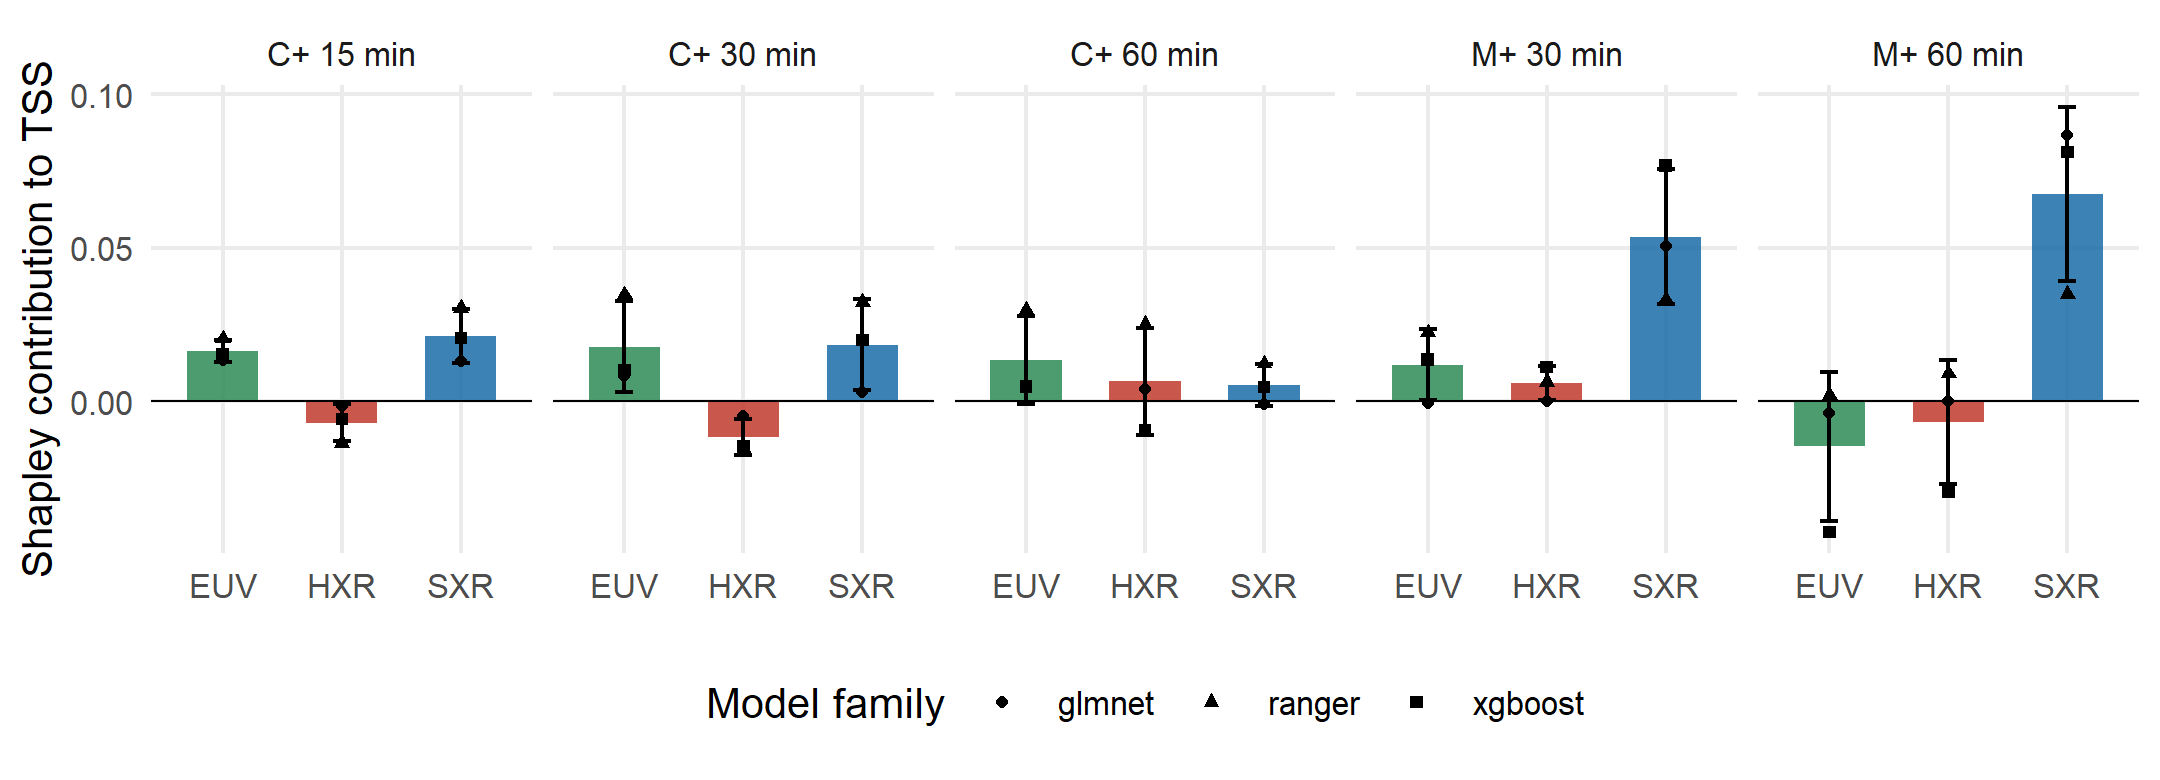
\includegraphics[width=0.78\textwidth]{fig_shapley_bands.png}
\caption{Shapley contribution of each band to pooled TSS beyond the baseline (leave-one-block-out). Bars: mean over the three model families, whiskers: $\pm$1 SD across families; markers: the individual families.}
\label{fig:shapley}
\end{figure*}

\subsection{What the alerts would look like}
Table~\ref{tab:alert} shows alert episodes for the boosted-tree model under LOO. For the C+ targets the full model raises \EpDayFullLo--\EpDayFullHi\ episodes per day and only \EpPrecFullLo--\EpPrecFullHi\% of them are followed by a flare, against \EpDayHistLo--\EpDayHistHi\ per day and \EpPrecHistLo--\EpPrecHistHi\% for the baseline model, which catches slightly fewer flares. For M+ targets, where alerts are rarer, only 18--37\% of episodes are followed by a flare (Table~\ref{tab:alert}). At the TSS-optimal threshold an alert is active \DutyLo--\DutyHi\% of all minutes. These forecasts cannot be used operationally as they stand. A real alert policy would have to pick its threshold for a target false-alarm rate, not for maximum TSS.

\begin{table}[t]
\caption{Alert episodes (boosted trees, leave-one-block-out): episodes per day, share followed by a flare, share of flares preceded by an alert, and share of minutes with an alert active.}
\label{tab:alert}
\centering\footnotesize
\begin{tabular}{llrrrr}
\toprule
Target & Features & Episodes/day & Precision & Flares caught & Alert on \\
\midrule
C+ 15 & History & 7.8 & 69\% & 38\% & 43\% \\
C+ 15 & All bands & 18.5 & 32\% & 40\% & 32\% \\
C+ 30 & History & 7.4 & 71\% & 37\% & 41\% \\
C+ 30 & All bands & 12.5 & 45\% & 38\% & 31\% \\
C+ 60 & History & 6.0 & 78\% & 33\% & 33\% \\
C+ 60 & All bands & 11.3 & 61\% & 42\% & 34\% \\
M+ 30 & History & 8.2 & 28\% & 52\% & 47\% \\
M+ 30 & All bands & 14.8 & 18\% & 59\% & 37\% \\
M+ 60 & History & 6.4 & 37\% & 49\% & 40\% \\
M+ 60 & All bands & 10.9 & 28\% & 58\% & 42\% \\
\bottomrule
\end{tabular}

\end{table}

\subsection{Robustness to SEP-contaminated periods}
\label{sec:robust}
We repeated the LOO analysis with the seven catalogued SEP-contamination periods \emph{included} (\NumSepMin\ additional minutes; logistic and boosted-tree families only). The pooled TSS of individual configurations changes by \SepMeanAbs\ on average and by at most \SepMaxAbs\ (Table~\ref{tab:sep}). The Shapley ranges across targets are SXR \SepShapLoSXR--\SepShapHiSXR, HXR \SepShapLoHXR--\SepShapHiHXR\ and EUV \SepShapLoEUV--\SepShapHiEUV, so the conclusion is unchanged: only SXR shows a positive contribution.

\begin{table}[t]
\caption{Sensitivity to SEP-contaminated periods: pooled TSS (mean of logistic and boosted-tree families) with the periods excluded (main analysis) or included.}
\label{tab:sep}
\centering\footnotesize
\begin{tabular}{llcc}
\toprule
Target & Features & SEP excluded & SEP included \\
\midrule
C+ 15 & History + magnetic & 0.08 & 0.08 \\
C+ 15 & All bands & 0.11 & 0.11 \\
C+ 30 & History + magnetic & 0.08 & 0.09 \\
C+ 30 & All bands & 0.09 & 0.11 \\
C+ 60 & History + magnetic & 0.09 & 0.10 \\
C+ 60 & All bands & 0.09 & 0.11 \\
M+ 30 & History + magnetic & 0.20 & 0.21 \\
M+ 30 & All bands & 0.28 & 0.28 \\
M+ 60 & History + magnetic & 0.22 & 0.21 \\
M+ 60 & All bands & 0.26 & 0.28 \\
\bottomrule
\end{tabular}

\end{table}

\section{Discussion}
\label{sec:disc}
\textbf{HXR helps with nowcasting, not forecasting.} The Neupert result and the earlier detection by HEL1OS show that HXR carries real information once a flare has started. As a forecaster it adds nothing steady, even with the 8~s features. This fits the physics: the non-thermal electrons are accelerated at the same moment the flare begins, so there is little to see beforehand. The hot soft X-ray onsets reported before the hard X-ray burst~\cite{hudson2021} are consistent with this. The small pre-flare brightenings seen by Aditya-L1~\cite{isro2026} would need a finer cadence than HEL1OS gives us.

\textbf{The validation design matters, especially with little data.} Leave-one-block-out uses data efficiently but lets the model learn from activity that comes later. Forward-in-time testing is the realistic estimate. It cut skill by 0.11 TSS in the two-month pilot and by \FwdDiffMean\ with six months, so the weaker design is less misleading once there is more data. Anyone forecasting flares from autocorrelated series should report the forward design.

\textbf{What the SXR gain means.} A single SoLEXS-level feature matches every band combination for M+ targets. That suggests the soft X-ray gain is mostly persistence: when the Sun is bright in soft X-rays, large flares are more likely. At one-minute cadence the bands therefore give little \emph{precursor} information, in line with earlier work on hot onsets~\cite{hudson2021}.

\textbf{Limitations.} Our window covers one phase of one solar cycle (\NumDays\ days, only \NumFlaresX\ X-class flares). The forward design has six test blocks and two model families, so its intervals are wide. The bootstrap holds models fixed; the paired-block analysis includes refit variability but has few blocks. No multiplicity correction is applied. Excluding minutes inside ongoing flares uses the flare end time, a hindsight that favours the models slightly. The magnetic block is a crude full-disk summary: it cannot say which region will flare, so finding that it adds nothing does not mean magnetic data are uninformative. One-minute averaging, and HEL1OS's 8~s readout, limit sensitivity to short precursors, and HEL1OS 60--150~keV is sensitive to particle background even outside catalogued periods. A preliminary analysis of 21 days of Fermi/GBM data (May 2024) used a single split and no history baseline and was inconclusive~\cite{techreport}; we draw no conclusions from it.

\section{Conclusion}
We used Aditya-L1 SoLEXS and HEL1OS data together with GOES EUV and SDO/HMI magnetic summaries, and kept two questions apart. For nowcasting, HEL1OS follows the SXR derivative in \NeuPos\% of M/X flares and shows them about a minute before SoLEXS when both detect them. For forecasting, once flare history and magnetic state are in the baseline, only the soft X-ray band helps consistently (about \FwdGainSXR\ TSS forward in time, most for M+ flares). A single soft X-ray level feature matches it, so it is largely persistence. HXR and EUV add nothing steady at this cadence, the full-disk magnetic summaries add nothing, and the alerts come too often to be useful. The natural next steps are a longer record covering more of the solar cycle, magnetic features resolved by region so that each band is measured on top of a state-of-the-art forecaster, and alert policies tuned to a target false-alarm rate.

\section*{Acknowledgment}
The study grew out of Problem Statement~15 of the Bharatiya Antariksh Hackathon 2026 (team TRiYana). Aditya-L1 SoLEXS and HEL1OS data were obtained from the ISRO Science Data Archive (ISSDC/PRADAN); GOES EUV and flare data from NOAA NCEI; SDO/HMI data from the JSOC.

\bibliographystyle{IEEEtran}
\begin{thebibliography}{99}
\bibitem{neupert1968} W.~M. Neupert, ``Comparison of solar X-ray line emission with microwave emission during flares,'' \emph{Astrophys. J. Lett.}, vol.~153, p.~L59, 1968.
\bibitem{dennis1993} B.~R. Dennis and D.~M. Zarro, ``The Neupert effect: What can it tell us about the impulsive and gradual phases of solar flares?'' \emph{Sol. Phys.}, vol.~146, pp.~177--190, 1993.
\bibitem{veronig2002} A.~Veronig, B.~Vr\v{s}nak, B.~R. Dennis, M.~Temmer, A.~Hanslmeier, and J.~Magdaleni\'c, ``Investigation of the Neupert effect in solar flares. I. Statistical properties and the evaporation model,'' \emph{Astron. Astrophys.}, vol.~392, pp.~699--712, 2002.
\bibitem{tripathi2022} D.~Tripathi \emph{et al.}, ``The Aditya-L1 mission of ISRO,'' arXiv:2212.13046, 2022.
\bibitem{nandi2025} A.~Nandi \emph{et al.}, ``HEL1OS -- A hard X-ray spectrometer on board Aditya-L1,'' \emph{Sol. Phys.}, vol.~300, p.~140, 2025.
\bibitem{bobra2015} M.~G. Bobra and S.~Couvidat, ``Solar flare prediction using SDO/HMI vector magnetic field data with a machine-learning algorithm,'' \emph{Astrophys. J.}, vol.~798, p.~135, 2015.
\bibitem{chen2019} Y.~Chen \emph{et al.}, ``Identifying solar flare precursors using time series of SDO/HMI images and SHARP parameters,'' \emph{Space Weather}, vol.~17, no.~10, 2019.
\bibitem{bloomfield2012} D.~S. Bloomfield, P.~A. Higgins, R.~T.~J. McAteer, and P.~T. Gallagher, ``Toward reliable benchmarking of solar flare forecasting methods,'' \emph{Astrophys. J. Lett.}, vol.~747, p.~L41, 2012.
\bibitem{barnes2016} G.~Barnes \emph{et al.}, ``A comparison of flare forecasting methods. I. Results from the `All-Clear' workshop,'' \emph{Astrophys. J.}, vol.~829, p.~89, 2016.
\bibitem{landa2022} V.~Landa and Y.~Reuveni, ``Low dimensional convolutional neural network for solar flares GOES time series classification,'' \emph{Astrophys. J. Suppl. Ser.}, vol.~258, p.~12, 2022.
\bibitem{gyenge2016} N.~Gyenge, I.~Ballai, and T.~Baranyi, ``Statistical study of spatio-temporal distribution of precursor solar flares associated with major flares,'' \emph{Mon. Not. R. Astron. Soc.}, vol.~459, pp.~3532--3539, 2016.
\bibitem{hudson2021} H.~S. Hudson, P.~J.~A. Sim\~oes, L.~Fletcher, L.~A. Hayes, and I.~G. Hannah, ``Hot X-ray onsets of solar flares,'' \emph{Mon. Not. R. Astron. Soc.}, 2021, doi:10.1093/mnras/staa3664.
\bibitem{isro2026} ISRO, ``Aditya-L1 catches the Sun's early warning signs before solar flares,'' press release, Aug.\ 2026. [Online]. Available: https://www.isro.gov.in
\bibitem{scherrer2012} P.~H. Scherrer \emph{et al.}, ``The Helioseismic and Magnetic Imager (HMI) investigation for the Solar Dynamics Observatory (SDO),'' \emph{Sol. Phys.}, vol.~275, pp.~207--227, 2012.
\bibitem{bobra2014} M.~G. Bobra \emph{et al.}, ``The Helioseismic and Magnetic Imager (HMI) vector magnetic field pipeline: SHARPs -- Space-weather HMI Active Region Patches,'' \emph{Sol. Phys.}, vol.~289, 2014, doi:10.1007/s11207-014-0529-3.
\bibitem{sepcat} HEL1OS Team, ``HEL1OS SEP Contamination-Times Catalog,'' Document HEL1OS-SEP-CAT-2026-V1.0, ISSDC/PRADAN, 2026.
\bibitem{shapley1953} L.~S. Shapley, ``A value for $n$-person games,'' in \emph{Contributions to the Theory of Games II}, Princeton Univ.\ Press, 1953, pp.~307--317.
\bibitem{techreport} A.~Abbabathula, ``Technical report: preliminary Fermi/GBM study,'' project repository, \texttt{report/report.html}, 2026.
\end{thebibliography}

\end{document}
